% !TEX root = 0_main.tex
\chapter{Introduction}
%what is the problem?
Secure function evaluation (SFE) allows two or more parties to correctly compute a function of their respective private inputs without exposure.
The seminal result by Yao introduced the GC protocol for addressing two-party SFE \cite{yao1986generate}.
The GC protocol allows to securely evaluate a function given as a Boolean circuit that is represented as a series of binary gates.
The inputs and outputs of each gate are masked such that the party evaluating the GC cannot gain any information about the inputs or  intermediate results that appear during function evaluation.
The approach of obliviously evaluating a Boolean circuit can also be generalized to multi-party SFE \cite{goldreich1987play,ben2008fairplaymp}.

%What has been done?
Contemporary literature has cited multiple important privacy preserving and security critical applications that could benefit from a practical realization of SFE, including but not limited to: biometrics matching, face recognition, image/data classification, electronic auctions and voting, remote diagnosis, and secure search \cite{bringer2013privacy, evans2011efficient, barni2009secure, naor1999privacy, brickell2007privacy, jha2008towards}.
While GC was considered to be prohibitively expensive and practically infeasible a decade ago, today we are witnessing a surge of theoretical, algorithmic, and tool developments that have significantly improved the efficiency and practicality of the GC protocol, see \cite{malkhi2004fairplay, kolesnikov2008improved, pinkas2009secure, huang2011faster, bellare2013efficient}.

%classification of the work
The research on producing Boolean functions for SFE can be roughly classified into two categories: optimizations of cryptographic constructs and protocols such as  \cite{kolesnikov2008improved,pinkas2009secure,bellare2012foundations,bellare2013efficient,kolesnikov2014flexor,zahur2015two}, and compiler/engineering techniques including but not limited to \cite{malkhi2004fairplay,kreuter2012billion,huang2011faster, malka2011vmcrypt,henecka2013faster,kreuter2013pcf,franz2014cbmc}.

In the compiler/engineering realm two different approaches for circuit generation have been developed.
One approach is based on building a custom library for a general purpose programming language such as Java along with functions for emitting the circuit, e.g., \cite{huang2011faster,malka2011vmcrypt,henecka2013faster}.
For better usability, these libraries typically include frequently used modules such as adders and multipliers.
However, library-based approaches require manual adjustment and do not perform global circuit optimization.
Moreover, their memory management gets complicated when the number of gates is large thereby affecting performance and scalability \cite{henecka2013faster}.

The second approach is to write a new compiler for a higher-level language that translates the instructions into the Boolean logic, e.g., \cite{malkhi2004fairplay,kreuter2012billion,kreuter2013pcf,franz2014cbmc}.
Although compiler-based approaches can perform global optimizations, they often unroll the circuits into a large list of gates.
For example, the description of a circuit with one billion gates has at least size $2 \log_2 (10^9) \cdot 10^{9} \approx 7$~GB.
To reduce circuit description size, the compiler proposed in \cite{kreuter2013pcf}, called PCF (Portable Circuit Format), does not unroll the loops in the circuit until the GC protocol runs, and therefore seems to have a better scalability than the other compilers.
As we elaborate in related work (see \sect{sect:related}), the existing approaches, including the above proposals, have certain limitations when it comes to real implementation.

Our approach, TinyGarble, is based on synthesizing and optimizing circuits for the GC protocol as sequential circuits while leveraging powerful logic synthesis techniques with our newly introduced custom-libraries.

Our solution simply views the circuit generation for GC as an atypical logic synthesis task that, if properly defined, can still be addressed by conventional hardware synthesis tools.
By posing the circuit generation for Yao's protocol as a hardware synthesis problem, TinyGarble naturally benefits from the elegant algorithms and powerful techniques already incorporated in existing logic synthesis solutions, see, \cite{sentovich1992sis,micheli1994synthesis,devadas1994logic,brayton1987mis}.
This view provides a radically different perspective on this important problem in contrast to the earlier work in this area that attempted to generate circuits by building new libraries for general purpose languages such as Java \cite{huang2011faster,malka2011vmcrypt}, custom compilers such as \cite{kreuter2013pcf,franz2014cbmc}, or introduction of new programming languages such as \cite{malkhi2004fairplay,rastogi2014wysteria}.

TinyGarble introduces new techniques for minimizing the number of non-XOR gates which directly results in reduced computation and communication required for the GC protocol.
We do so by integrating the cost function in the new custom libraries that we design and use within our logic synthesis flow.
This way, we are able to gain up to $80\%$ improvement in the number of non-XOR gates for benchmark circuits compared to PCF \cite{kreuter2013pcf}.
The TinyGarble methodology is automated, i.e., the savings can be achieved for many functions synthesized by our method, regardless of their sophistication.

One significant contribution of TinyGarble, which differentiates it from the previous work, is expressing the function in a very compact format, namely as a sequential logic.
The earlier work in this area mainly described functions in a combinational format, where the value of the output is determined entirely by the circuit inputs.
This input/output relationship can be expressed by a (combinational) Boolean function and a directed acyclic graph (DAG) of binary gates.
The sequential circuit description, on the other hand, allows having feedback from the output to the input by adding the notion of a state (memory).
At each \emph{sequential cycle}, the output of the circuit is determined by the current state of the system and the input.
For each particular sequential cycle, the relationship between the output and the inputs for the given states can be determined as a Boolean combinational logic.

The only previous work we are aware of which implicitly hinted at the possibility of having a more compact representation is PCF \cite{kreuter2013pcf}.
It does so by embracing loops and unrolling them only at runtime.
A sequential circuit, however, goes far beyond the loop embracing performed at the software level.
Not only does TinyGarble embrace the high-level loops, it also enables the user to further compact the functions by folding the implementation up to its basic elements.
For example, using TinyGarble, user can compress the 1024-bit addition function into only a 1-bit adder.

An important advantage of our sequential representation is providing a new degree of freedom to the user to fold the functions to simpler computing elements; i.e., the user has the freedom to choose the number of sequential cycles needed for evaluation of the function--the size of the combinational logic path between the states/inputs and the outputs.
The number of gates in the sequential circuit can be managed by varying the number of cycles.
The memory footprint of the GC operation is directly related to the number of gates in the sequential circuit; at any moment during garbling, only the information corresponding to the current cycle needs to be stored.
Compact sequential circuits yield a small enough memory footprint that can fit mostly on a typical processor cache.
This helps us to avoid costly cache misses while accessing the wire tokens during the GC protocol.
Indeed, TinyGarble can enable practicable embedded implementations with a small memory footprint.

The sequential representation enables, for the first time, implementation of a universal processor for private function evaluation where the function is known only to one party.
We reduce private function SFE (PF-SFE) to general SFE where the function is known by both parties.
Our implementation accepts assembly instructions of the private function as input to the GC protocol.
Since a processor is inherently a sequential circuit, it was infeasible to be realized with previous GC tools.

TinyGarble accepts inputs in two different formats: a standard hardware description language (HDL), or a higher level language as long as it is compatible with the existing high level synthesis (HLS) tools, e.g., the C language for  SPARK \cite{Gupta2004} and Xilinx Vivado \cite{tool:Vivado}, or Python for PandA \cite{tool:PandA}, that converts the high level language to an HDL.
Beside user's manual optimization, TinyGarble performs various optimizations through standard HDL synthesis tools to generate an optimized \emph{netlist}, i.e., list of gates, which is then transformed to be used with a GC protocol implementation, e.g., JustGarble \cite{bellare2013efficient} or Half Gates \cite{zahur2015two}.

%%%%%

Secure Function Evaluation (SFE) allows two (or more) mistrusting parties to jointly compute an arbitrary function on their private inputs without revealing information but the result. The seminal work of Yao \cite{yao1986generate} has introduced the concept of two-party SFE using the Garbled Circuits (GC) protocol which requires that the function is represented as a Boolean circuit. While the GC protocol was originally thought to be of theoretic interest only, algorithmic and implementation optimizations have significantly improved its efficiency during the last decades. In addition to the advances in computing platforms, the key enablers for the progress include newer cryptographic constructs, logic-level transformations, and software techniques.

Compilers for SFE have been continually evolving. A number of compilers~\cite{malkhi2004fairplay,ben2008fairplaymp,henecka2010tasty,kreuter2012billion} translate a functionality written in a domain-specific input language into a Boolean circuit, also described in an intermediate language, which is then evaluated with Yao's GC protocol. Other compilers \cite{franz2014cbmc,kreuter2013pcf} use a subset of the C language as input. However, these methods imply building software-to-Boolean circuit compilers from scratch and often put limitations on the functionality. Moreover, verifying the correctness of these compilers is challenging \cite{mood2016frigate}.

Recently, it was shown that the long-established and verified hardware synthesis compilers can be used for generation of Boolean circuits for SFE, eliminating the need for building ad-hoc logic compilers or tedious handcrafting of Boolean circuits. Another key advantage of conventional logic synthesis is allowing a \emph{sequential logic description} which can be adapted to map general functionalities to Boolean circuits optimized for Yao's GC protocol. The approach was introduced in \cite{songhori2015tinygarble} and shown to yield great improvements in terms of memory and communication. A fully-automated toolchain which utilizes existing logic synthesis compilers and can be generalized for other SFE protocols was presented in \cite{demmler2015automated}. This latter work takes advantage of the built-in intellectual property (IP) and custom design libraries which can be readily adapted during circuit synthesis to realize a broad suite of applications optimized for SFE.

The authors in \cite{songhori2015tinygarble} leverage the capability of synthesizing a sequential circuit and introduce the idea of a general-purpose sequential processor for private function SFE (PF-SFE) by GC, where both input data and function are private. PF-SFE is useful for scenarios where the function is proprietary or classified, e.g., credit checking or private database queries. Their so-called \emph{garbled processor} allows to use existing software compilers for describing the function and generates compatible machine code which is also garbled. A partial implementation of a MIPS processor is provided in \cite{songhori2015tinygarble} which only considers PF-SFE where the entire processor circuit and Instruction Set (IS) have to be garbled in each instruction step during SFE in order to hide the executed instructions in the private function. This results in a tremendous cost compared with SFE for public functions. Thus, their MIPS processor incurs an unnecessary overhead for numerous applications in which a private function is not required. (The only benchmark presented in \cite{songhori2015tinygarble} is the Hamming distance function.)

We propose GarbledCPU, the first configurable hardware-based general purpose sequential CPU for SFE. The FPGA realization of GarbledCPU is based on the MIPS instruction set. GarbledCPU provides a generalized support for SFE of varying flavors of privacy, beyond PF-SFE, to allow for more relaxed privacy demands and hence an improved performance. More explicitly, with GarbledCPU the parties can evaluate a private, semi-private or public function by revealing none, partial or all information about the function respectively while still benefiting from the simplicity of programming a processor.
Both parties decide first which subset of IS they are willing to use which determines the level of privacy ensured. The function is compiled from a high-level language, e.g., C/C++ into assembly code of the agreed upon IS. Next, the garbled processor is securely evaluated given users' garbled input and the compiled function instructions (also garbled) to compute the output.

A recent technical report \cite{wang2015secure} also suggests a secure computation framework using MIPS code. The approach relies on garbled universal circuits to emulate the execution of each instruction of the MIPS program and on Oblivious RAM (ORAM) for memory access. They propose using static analysis of functions to reduce the set of instructions to be garbled. However, \cite{wang2015secure} only presents a software SFE implementation, while we present the first practical hardware sequential processor for both SFE and PF-SFE. An earlier hardware implementation of GC was reported in \cite{jarvinen2010garbled} but the approach only addresses SFE with no support for function hiding and is limited to combinational Boolean circuit as it predated \cite{songhori2015tinygarble}. A combinational description limits usability and scalability and is impractical for control-intensive functions such as CPUs that need to be expressed sequentially.

%%%%%

Secure Function Evaluation (SFE) allows two or more parties to compute an arbitrary joint function such that they learn the function output without revealing their private inputs.
The first and by far the most efficient method for two-party SFE is Yao's Garbled Circuit (GC) protocol~\cite{yao1986generate}.
Yao's protocol immediately attracted a significant attention from the cryptography community, but was believed to be of limited practical usage for many years.
The critical challenge of GC was to generate an optimized Boolean circuit representing the function such that its secure evaluation incurs the minimum communication and encryption cost.

The GC logic optimization challenge was recently addressed by TinyGarble~\cite{songhori2015tinygarble}.
Even though the circuit is just a Boolean representation to be used in GC, a software protocol, TinyGarble showed that the circuit generation can be viewed as an atypical instance of the conventional logic synthesis task.
This approach outperforms previous methods for generating Boolean circuit using custom compilers~\cite{malkhi2004fairplay,holzer2012secure, rastogi2014wysteria,demmler2015aby,liu2015oblivm,mood2016frigate}.
A major disadvantage of TinyGarble, however, is that the efficiency can only be achieved when the function is described in a Hardware Description Language (HDL), e.g., Verilog, instead of a high-level programming language.
Even when they used the best high-level synthesis compiler, i.e., Vivado HLS ~\cite{tool:Vivado}, they lost the HDL efficiency.
In this paper, our goal is to combine the efficiency of hardware synthesis with the versatility of high-level languages.

Recently, a number of researchers proposed the idea of \textit{garbled processor} where the underlying Boolean circuit in GC is that of a general-purpose processor~\cite{wang2015secure, songhori2016garbledcpu}.
This way, users can develop the secure function in a high-level language and feed the compiled binary code to the processor along with their private inputs.
However, the large overheads of such approaches compared with the classic HDL synthesis raises questions about their practicality.
We believe that the primary reason behind the overhead is that they perform coarse-grain (instruction-level) optimization.
At each cycle, they generate a custom processor supporting only the instruction(s) to be executed at that cycle.

In this work, we introduce a methodology to perform fine-grain (gate-level) optimization on garbled processor such that only the gates associated to the private inputs incur garbling cost.
Our key observation is that the gates whose outputs are independent of the private data (and thus known to both parties) can either be computed without communication and encryption or simply skipped.
This observation gives birth to the novel SkipGate algorithm.
The algorithm wraps around the GC protocol to compute the gate outputs that can be computed without communication and to mark the redundant gates for skipping\footnote{SkipGate avoids garbling redundant gates and is orthogonal to cryptographic methods such as Free XOR~\cite{kolesnikov2008improved} and Half Gate~\cite{zahur2015two} that reduce the garbling cost of a gate.}.

SkipGate is mostly effective for reducing the garbling cost of sequential circuits~\cite{songhori2015tinygarble} containing known control paths.
An example of such a circuit is the garbled processor where the control path depends on the binary code of the function that is known to both parties.
By utilizing this property, we develop a high-level GC framework called ARM2GC built upon the ARM instruction set and the SkipGate algorithm.
Users can develop the secure function in high-level languages, e.g., C/C++ and compile it using standard ARM cross-compilers.
In contrast to the earlier custom high-level compilers which called for new ad-hoc verification techniques~\cite{rastogi2014wysteria,demmler2015aby,liu2015oblivm,mood2016frigate}, ARM2GC inherits the ARM's available fully verified compilers.
Thanks to SkipGate, ARM2GC incurs a garbling cost comparable to the HDL synthesis approach of TinyGarble while allowing users to develop SFE applications in a high-level language.

Our work leverages ARM as the general purpose processor, in contrast to the earlier MIPS-based garble processors~\cite{songhori2015tinygarble, wang2015secure, songhori2016garbledcpu} because of ARM's pervasiveness and, most importantly, conditional execution.
The latter simplifies the framework by reducing conditional branches and making the program flow predictable for both parties to take the full advantage of the SkipGate algorithm.
We modify the standard ARM architecture (without affecting the instruction set) such that SkipGate is more effective on the circuit.

\section{Contributions}
\paragraph*{Contributions} In brief, our contributions are as follows:
\begin{itemize}
\item We propose the first hardware-only solution for 2-party GC-based secure sequential function computation with different SFE flavors that allows leveraging the trade-off between privacy and performance: application-specific IS for SFE (\sect{ssect:sfe}), restricted IS (\sect{ssect:semi-pf}) for semi-private SFE, and full IS (\sect{ssect:pfsfe}) for PF-SFE.
\item We realize a proof-of-concept FPGA implementation which demonstrates the feasibility of the sequential garbled processor in hardware, and motivates further research in this direction. GarbledCPU achieves efficiency and performance by leveraging the most recent optimizations for GC \cite{kolesnikov2008improved,bellare2013efficient,zahur2015two,songhori2015tinygarble}, along with a high-throughput pipelined GC evaluation on FPGA. It outperforms the fastest software implementation in the literature which relies on the Intel AES-NI \cite{bellare2013efficient}.
\item We extensively benchmark more complex functions such as AES, Private Set Intersection (PSI), and Hamming distance and evaluate them under our different privacy settings using our framework and when applicable, compare our performance with prior work.
\item We introduce the novel SkipGate algorithm that avoids redundant garbling by utilizing the mutual knowledge between the two parties.
\item
  Adaption of established HDL synthesis techniques to compile and optimize a function into a netlist of gates for use in secure computation protocols.
\item
  Creation of new custom libraries and setting objectives/ constraints to \emph{repurpose} standard synthesis tools for minimizing the number of non-XOR gates in a circuit.
\item
  Introduction of sequential circuit description for achieving an unprecedented compactness in function representation and memory footprint.
\item
  Providing a new degree of freedom to users to fold the functions into a sequential circuit.
  The user can achieve a small enough sequential circuit such that the memory required for its secure evaluation fits even in a typical processor cache.
  This helps to avoid costly cache misses and reduces the CPU time required for GC.
\item
  Proof-of-concept implementation of benchmark functions such as multiplication, and Hamming distance demonstrates up to 5 orders of magnitude savings in memory footprint and up to $80\%$ efficiency in minimizing the total number of non-XOR gates.
  Furthermore, TinyGarble enables implementation of large circuits that were not reported in earlier work, such as SHA-3.% and RSA-8192.

\item
  Implementing the first scalable emulation of a universal processor for private function evaluation where the number of instruction invocations is not limited by the memory required for garbling.
  This design is uniquely enabled by the TinyGarble sequential description.
  Our design is a secure general purpose processor based on the MIPS~I instruction set that receives as inputs the private function from one party and the data from the other.
\item We develop the ARM2GC framework based on the SkipGate algorithm and ARM processor.
    In this framework, users can efficiently develop SFE applications in a high-level language like C/C++.
    It enables them to benefit from the available fully verified compilers of ARM.
    We modify the ARM architecture (without affecting the instruction set) to make it most effective for the GC protocol with SkipGate.
\item We perform extensive experiments to evaluate the SkipGate algorithm and the ARM2GC framework.
    The ARM2GC framework demonstrates comparable performance to HDL synthesis approach of TinyGarble~\cite{songhori2015tinygarble}.
    Its overhead is negligible for most of the benchmark functions and has the maximum value of 6\%.
    As expected, it outperforms the state-of-the-art garbled processors~\cite{wang2015secure, songhori2016garbledcpu} and high-level GC compilers~\cite{holzer2012secure, mood2016frigate}.
\end{itemize}

what we explained in hardware synthesis can be expand to other methods such GMW as shown in ~\cite{} however in this thesis we focus on the GC protocol.

\section{Global Flow}
The global flow of TinyGarble framework is shown in \fig{fig:globalflow}.
The framework consists of two main part (i) GC synthesis and (ii) GC engine.
The GC synthesis flow (\chap{chap:syn}) receives a function description in HDL and generates a circuit description that can be efficiently evaluated by the GC engine.
The GC engine is the implementation of Yao's GC protocol in C++ and is developed based on JustGarble \cite{bellare2013efficient}.
Our GC engine supports communication which was missing in JustGarble.
It also includes implementation of Half Gate \cite{zahur2015two}, the most recent optimization on the GC protocol that reduces the communication and computation cost by 33\%.
The engine also supports garbling/evaluating sequential circuits (\chap{chap:seq}) and SkipGate algorithm to reduce the sequential circuit overhead (\chap{chap:skipgate}).

\begin{figure}[ht]
\centering
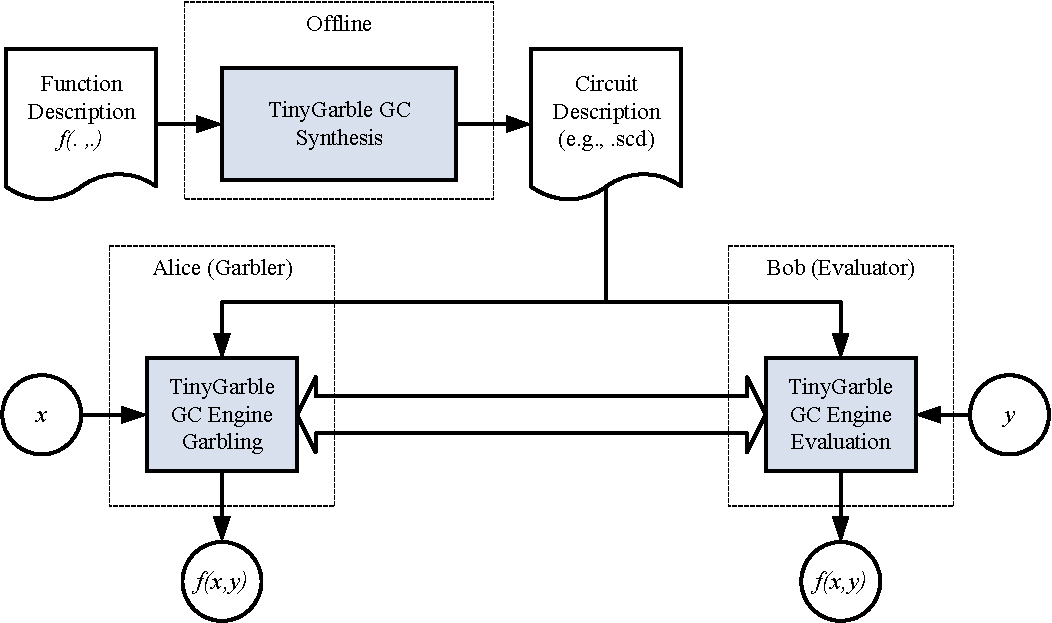
\includegraphics[width=0.95\textwidth]{TinyGarble_flow-crop.pdf}
\caption{The global flow of TinyGarble framework.
The framework consists of GC synthesis flow and GC engine.
The GC synthesis flow generates the optimized circuit description given a function.
The GC engine implements the Yao's GC protocol for both garbler and evaluator.
}
\label{fig:globalflow}
\end{figure}

\section{Organization}
